\documentclass[tikz,multi=tikzpicture,border=7pt]{standalone}
\usepackage{ctex}
\usepackage{amsmath,amssymb,bm}
\usetikzlibrary{arrows.meta,calc,decorations.pathmorphing,patterns,positioning,angles,quotes,3d}
\tikzset{
  vec/.style={-{Latex[length=2.6mm]},very thick,blue!72!black},
  impulse/.style={-{Latex[length=2.8mm]},very thick,red!72!black},
  guide/.style={gray!70,dashed},
  body/.style={draw,very thick,fill=blue!7},
  charge/.style={circle,draw,very thick,fill=orange!45,inner sep=2.2pt},
  nodept/.style={circle,draw,fill=white,inner sep=1.5pt},
  dim/.style={<->,>=Latex,thin},
  resistor/.style={decorate,decoration={zigzag,segment length=4pt,amplitude=2pt},thick}
}
\tikzset{vec/.style={-{Latex[length=2.4mm]},very thick,blue!70!black},force/.style={-{Latex[length=2.4mm]},very thick,red!70!black},impulse/.style={force},ray/.style={-{Latex[length=2.2mm]},thick,orange!80!black},wave/.style={blue!70!black,thick},body/.style={draw,very thick,fill=blue!7},guide/.style={gray!65,dashed},dim/.style={<->,>=Latex,thin},resistor/.style={decorate,decoration={zigzag,segment length=4pt,amplitude=2pt},thick}}
\begin{document}

% 1 question-01
\begin{tikzpicture}[font=\small,x=1cm,y=1cm]
  \draw[very thick,->] (-5.8,0)--(5.8,0) node[right] {切向 $x$（库边）};
  \draw[->] (0,-.6)--(0,3.7) node[above] {法向 $y$};
  \draw[vec] (-3.1,3.1)--(0,0) node[midway,above right] {$\bm v_0$};
  \draw[vec] (0,0)--(-1.55,2.685) node[midway,above left] {$\bm v'$};
  \draw (0,.72) arc (90:135:.72) node[midway,above left] {$\theta$};
  \draw (0,.72) arc (90:120:.72) node[midway,above right] {$\alpha=-30^\circ$};
  \begin{scope}[shift={(4.45,2.85)}]
    \shade[ball color=blue!18] (0,0) circle (.72);
    \draw[impulse] (-.5,.5) arc (135:445:.72) node[above right] {$\omega_0$};
    \fill[red!70!black] (-.45,-.55) circle (2pt);
    \node[below] at (0,-.9) {俯视球—库接触};
  \end{scope}
\end{tikzpicture}

% 2 solution-01
\begin{tikzpicture}[x=1cm,y=1cm,font=\small]

\begin{scope}[shift={(-3.8,0)}]
\draw[->] (-2.8,0)--(2.8,0) node[right] {$t$};\draw[->] (0,-.8)--(0,3) node[above] {$n$};
\draw[vec] (-2,2)--(0,0) node[midway,left] {$v_0$};
\draw[vec] (0,0)--(-1.3,2.25) node[above left] {$\alpha=-30^\circ$};
\draw[impulse] (0,0)--(0,1.6) node[right] {$J_n$};\draw[impulse] (0,0)--(-2.4,0) node[below] {$J_t$};
\node at (0,-1.5) {$v_t'=v_t-J_t/m<0$};
\end{scope}
\begin{scope}[shift={(3.8,.4)}]
\draw[very thick] (-2.7,-1.1)--(2.7,-1.1);\draw[body] (0,0) circle (1.1);
\fill (0,-1.1) circle (2pt) node[below] {$P$};\draw[vec] (0,.15)--(2,.15) node[right] {$v_t$};
\draw[impulse] (.8,.8) arc (45:315:1.13);\node at (0,1.6) {$\omega>0$：逆时针};
\draw[impulse] (0,-1.1)--(-2,-1.1) node[left] {$J_t$};
\node at (0,-2) {$u_P=v_t+R\omega$};\node at (0,-2.65) {$\Delta K=-J_tu_P+\tfrac12J_t^2(1/m+R^2/I)$};
\end{scope}
\end{tikzpicture}

% 3 question-02
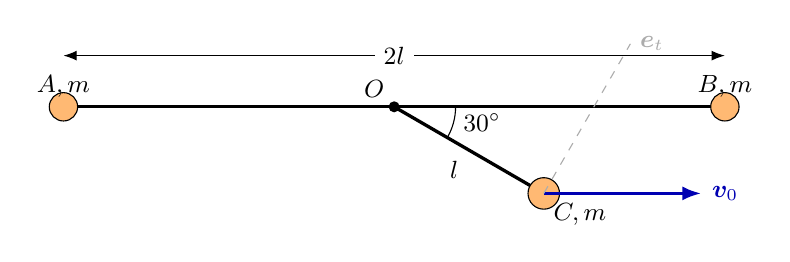
\begin{tikzpicture}[font=\small,x=1cm,y=1cm]
  \coordinate (O) at (0,1.1); \coordinate (A) at (-4.2,1.1); \coordinate (B) at (4.2,1.1); \coordinate (C) at (1.9,-.0);
  \draw[very thick] (A)--(B);
  \filldraw[fill=orange!55] (A) circle (.18) node[above] {$A,m$};
  \filldraw[fill=orange!55] (B) circle (.18) node[above] {$B,m$};
  \fill (O) circle (2pt) node[above left] {$O$};
  \draw[very thick] (O)--(C) node[midway,below left] {$l$};
  \filldraw[fill=orange!55] (C) circle (.2) node[below right] {$C,m$};
  \draw[vec] (C)--++(2.0,0) node[right] {$\bm v_0$};
  \draw[dim] ($(A)+(0,.65)$)--($(B)+(0,.65)$) node[midway,fill=white] {$2l$};
  \draw (O)+(.78,0) arc (0:-30:.78) node[midway,right] {$30^\circ$};
  \draw[guide] (C)--($(C)!1.0!-90:(O)$) node[right] {$\bm e_t$};
\end{tikzpicture}

% 4 solution-02
\begin{tikzpicture}[x=1cm,y=1cm,font=\small]

\begin{scope}[shift={(-4.5,1.4)}]
\coordinate(O)at(0,0);\coordinate(C)at(1.73,-1);
\draw[very thick](-2,0)--(2,0);\draw[very thick](O)--(C);
\foreach\p/\lab in {(-2,0)/A,(2,0)/B,(0,0)/O,(1.73,-1)/C}{\fill\p circle(2pt)node[below]{$\lab$};}
\draw[impulse](C)--++(-.86,.5)node[midway,above]{$J$};\draw[impulse](O)--++(.86,-.5)node[below]{$J$};
\draw[vec](C)--++(1.3,0)node[right]{$v_0$};\node at(0,-2){绷直瞬间：$J=mv_0/\sqrt3$};
\end{scope}\begin{scope}[shift={(2.5,1.5)}]\draw[very thick] plot coordinates {(-1.00000,-0.00000) (1.00000,0.00000)};
\fill (-1.00,-0.00) circle(2pt) node[left] {$A$};
\fill (1.00,0.00) circle(3pt) node[right] {$B,C$};
\node at(0,-1.7) {$\theta=0$};\end{scope}\begin{scope}[shift={(5.9,1.5)}]\draw[very thick] plot coordinates {(-0.00000,-1.00000) (0.00000,1.00000)};
\fill (-0.00,-1.00) circle(2pt) node[left] {$A$};
\fill (0.00,1.00) circle(3pt) node[right] {$B,C$};
\node at(0,-1.7) {$\theta=\pi/2$};\end{scope}\begin{scope}[shift={(2.5,-1.9)}]\draw[very thick] plot coordinates {(1.00000,-0.00000) (-1.00000,0.00000)};
\fill (1.00,-0.00) circle(2pt) node[left] {$A$};
\fill (-1.00,0.00) circle(3pt) node[right] {$B,C$};
\node at(0,-1.7) {$\theta=\pi$};\end{scope}\begin{scope}[shift={(5.9,-1.9)}]\draw[very thick] plot coordinates {(0.00000,1.00000) (-0.00000,-1.00000)};
\fill (0.00,1.00) circle(2pt) node[left] {$A$};
\fill (-0.00,-1.00) circle(3pt) node[right] {$B,C$};
\node at(0,-1.7) {$\theta=3\pi/2$};\end{scope}
\node[align=left]at(-4.5,-2.3){相邻两幅相隔 $4\pi l/v_0$\\中间各发生一次 $CA$ 碰撞\\四组后复原：$T=16\pi l/v_0$};
\end{tikzpicture}

% 5 question-03
\begin{tikzpicture}[font=\small,x=1cm,y=1cm]
  \def\s{2.0}
  \foreach \a in {0,60,...,300}{\coordinate (T\a) at ({sqrt(3)*\s*cos(\a)},{sqrt(3)*\s*sin(\a)});}
  \foreach \a in {30,90,...,330}{\coordinate (V\a) at ({\s*cos(\a)},{\s*sin(\a)});}
  \draw[very thick,fill=blue!8] (T0)--(V30)--(T60)--(V90)--(T120)--(V150)--(T180)--(V210)--(T240)--(V270)--(T300)--(V330)--cycle;
  \foreach \a in {30,90,...,330}{\draw[guide] (0,0)--(V\a);}
  \node[right] at (T0) {$B$}; \node[above right] at (T60) {$C$}; \node[above left] at (T120) {$D$};
  \node[left] at (T180) {$E$}; \node[below left] at (T240) {$F$}; \node[below right] at (T300) {$A$};
  \fill (0,0) circle (2.2pt) node[above left] {$O$};
  \draw[very thick] (-5,-3.0)--(5,-3.0) node[right] {地面};
  \draw[impulse] (T60)--++(2.4,0) node[right] {$I$};
  \draw[dim] (V30)--(V90) node[midway,above right] {$l$};
\end{tikzpicture}

% 6 solution-03
\begin{tikzpicture}[font=\small,x=1cm,y=1cm]
  \begin{scope}[shift={(-4.1,0)}]
    \coordinate (A) at (0,-2.5); \coordinate (O) at (-1.5,.10); \coordinate (C) at (0,2.5);
    \draw[very thick] (-3.2,-2.5)--(2.8,-2.5); \draw[guide] (A)--(O)--(C);
    \fill (A) circle (2pt) node[below] {$A$}; \fill (O) circle (2pt) node[left] {$O$}; \fill (C) circle (2pt) node[above] {$C$};
    \draw[impulse] (C)--++(2.0,0) node[right] {$I$};
    \draw[impulse] (A)--++(0,1.45) node[right] {$I_y$};
    \draw[vec] (O)--++(1.3,.75) node[right] {$\bm V_O$};
    \draw[impulse] (-.55,.95) arc (120:-45:1.0) node[right] {$\omega$};
    \node at (-.2,-3.25) {$OA=\sqrt3l,\quad AC=3l$};
  \end{scope}
  \begin{scope}[shift={(4.1,-.3)}]
    \coordinate (A) at (0,-2.2); \coordinate (O) at (-1.35,.14);
    \draw[very thick] (-3,-2.2)--(3,-2.2); \draw[very thick] (A)--(O);
    \draw[guide] (A)--(0,1.2);
    \draw (A)+(0,.85) arc (90:120:.85) node[midway,above] {$\alpha$};
    \fill (A) circle (2pt) node[below] {$A$}; \fill (O) circle (2pt) node[left] {$O$};
    \draw[impulse] (O)--++(0,-1.55) node[right] {$12mg$};
    \draw[dim] (A)+(-1.5,0)--++(3,0) node[right] {$F$（带符号）}; \draw[vec] (A)--++(0,1.45) node[right] {$N$};
    \node at (0,-3.0) {绕 $A$ 翻越时检验能量、$N\ge0$ 与 $|F|\le\mu N$};
  \end{scope}
\end{tikzpicture}

% 7 question-04
\begin{tikzpicture}[font=\small,x=1cm,y=1cm]
  \draw[very thick] (-5,0)--(5,0); \draw[very thick] (0,0)--(0,3.0);
  \draw[very thick] (-4.2,0)--(-4.2,-1.05) (4.2,0)--(4.2,-1.05);
  \draw[body,rounded corners=16pt] (-5.1,-2.5) rectangle (-3.3,-1.0);
  \draw[body,rounded corners=16pt] (3.3,-2.5) rectangle (5.1,-1.0);
  \draw[blue!65,fill=blue!12] (-5.05,-2.45) rectangle (-3.35,-1.9);
  \draw[blue!65,fill=blue!12] (3.35,-2.45) rectangle (5.05,-1.9);
  \draw[very thick] (-4.55,-.38)--(-3.85,.38) (-3.85,-.38)--(-4.55,.38);
  \draw[very thick] (3.85,-.38)--(4.55,.38) (4.55,-.38)--(3.85,.38);
  \node at (-4.2,.7) {$S_1$}; \node at (4.2,.7) {$S_2$};
  \node[above] at (-2.4,0) {$l_1$}; \node[above] at (2.5,0) {$l_2$}; \node[right] at (0,1.6) {$l_3$};
  \node at (-4.2,-1.65) {水，$n_0$}; \node at (4.2,-1.65) {水，$n_0$};
  \node[above] at (0,3.0) {干燥大气};
\end{tikzpicture}

% 8 solution-04
\begin{tikzpicture}[font=\small,x=1cm,y=1cm]
  \node[nodept,label=below:左容器] (L) at (-4,0) {$n_0$};
  \node[nodept,label=below:汇合点] (P) at (0,0) {$n_p$};
  \node[nodept,label=below:右容器] (R) at (4,0) {$n_0$};
  \node[nodept,label=right:干燥端] (D) at (0,3) {$0$};
  \draw[very thick] (L)--(P) node[midway,above=4pt] {$DS/l_1$};
  \draw[very thick] (R)--(P) node[midway,above=4pt] {$DS/l_2$};
  \draw[very thick] (P)--(D) node[midway,right] {$DS/l_3$};
  \draw[impulse] (-2.9,.25)--(-1.1,.25); \draw[impulse] (2.9,.25)--(1.1,.25); \draw[impulse] (.25,.8)--(.25,2.2);
  \node at (0,-1.5) {$\dfrac{n_0-n_p}{l_1}+\dfrac{n_0-n_p}{l_2}=\dfrac{n_p}{l_3}$};
\end{tikzpicture}

% 9 question-05
\begin{tikzpicture}[font=\small,x=1cm,y=1cm]
  \draw[very thick] (-5.6,0)--(5.6,0); \draw[pattern=north east lines,draw=none] (-5.6,-.28) rectangle (5.6,0);
  \draw[very thick,fill=blue!7] (-2.0,0) arc (180:0:2.0)--cycle;
  \draw[->] (0,-.7)--(0,4.6) node[above] {$z$}; \draw[->] (-5.2,0)--(5.5,0) node[right] {$x$};
  \coordinate (Q) at (2.7,3.25); \draw[very thick] (0,0)--(Q) node[midway,right] {$a$};
  \node[charge] at (Q) {$q$};
  \draw (0,1.0) arc (90:50.2:1.0) node[midway,above right] {$\theta_0$};
  \draw[dim] (0,-.55)--(2,-.55) node[midway,below] {$R$};
  \node at (-3.7,.55) {接地导体平面}; \node at (3.8,1.2) {真空};
\end{tikzpicture}

% 10 solution-05
\begin{tikzpicture}[font=\small,x=1cm,y=1cm]
  \draw[very thick] (-5.5,0)--(5.5,0); \draw[very thick] (-1.75,0) arc (180:0:1.75);
  \draw[->] (0,-3.7)--(0,4.4) node[above] {$z$};
  \draw[guide] (0,0)--(2.7,3.15) (0,0)--(2.7,-3.15);
  \node[charge] (q1) at (2.7,3.15) {$q$};
  \node[charge,fill=red!18] (q2) at (2.7,-3.15) {$-q$};
  \node[charge,fill=red!18] (q3) at (.82,.96) {$-qR/a$};
  \node[charge] (q4) at (.82,-.96) {$qR/a$};
  \draw[dim] (0,.2)--(.82,1.16) node[midway,left] {$R^2/a$};
  \node[align=left] at (-3.65,2.2) {平面镜像保证 $z=0$ 势为零\\球面反演像保证 $r=R$ 势为零};
  \draw[vec] (-4.35,-1.35)--(-4.35,.55) node[above] {$\bm p\parallel\hat{\bm z}$};
\begin{scope}[shift={(-3.8,-2.2)}]
\draw[very thick] (0,0) ellipse(1.1 and .35);\draw[impulse](1.1,0) arc(0:160:1.1 and .35);
\node[below,align=center]at(0,-.6){仅有 $\oint B_\varphi\,\mathrm dl=0$\\不能推出逐点 $B_\varphi=0$};\end{scope}\end{tikzpicture}

% 11 question-06
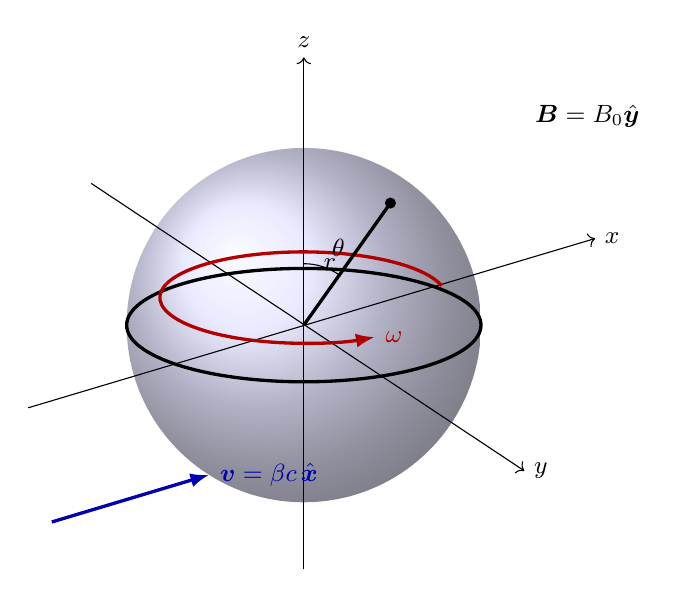
\begin{tikzpicture}[font=\small,x=1cm,y=1cm]
  \shade[ball color=blue!15,opacity=.75] (0,0) circle (2.25);
  \draw[very thick] (0,0) ellipse (2.25 and .72);
  \draw[->] (0,-3.1)--(0,3.4) node[above] {$z$};
  \draw[->] (-3.5,-1.05)--(3.7,1.1) node[right] {$x$};
  \draw[->] (-2.7,1.8)--(2.8,-1.85) node[right] {$y$};
  \draw[impulse] (1.75,.5) arc (15:300:1.82 and .58) node[right] {$\omega$};
  \coordinate (P) at (1.1,1.55); \fill (P) circle (2pt); \draw[very thick] (0,0)--(P) node[midway,left] {$r$};
  \draw (0,.78) arc (90:55:.78) node[midway,above right] {$\theta$};
  \draw[vec] (-3.2,-2.5)--(-1.2,-1.9) node[right] {$\bm v=\beta c\,\hat{\bm x}$};
  \node at (3.6,2.65) {$\bm B=B_0\hat{\bm y}$};
\end{tikzpicture}

% 12 solution-06
\begin{tikzpicture}[font=\small,x=1cm,y=1cm]
  \begin{scope}[shift={(-3.8,0)}]
    \draw[very thick,fill=blue!6] (0,0) ellipse (1.35 and 2.25);
    \draw[->] (-2.3,0)--(2.4,0) node[right] {$x'$}; \draw[->] (0,-2.8)--(0,2.9) node[above] {$z'$};
    \draw[vec] (0,0)--(.85,1.3) node[right] {$\bm n'$};
    \node at (0,-3.35) {$x'^2/(r/\gamma)^2+y'^2/r^2+z'^2/r^2=1$};
  \end{scope}
  \begin{scope}[shift={(3.7,0)}]
    \draw[->] (-2.2,0)--(2.5,0) node[right] {$y'$}; \draw[->] (0,-2.4)--(0,2.6) node[above] {$z'$};
    \draw[vec] (0,0)--(0,1.65) node[left] {$\bm m_{\mathcal M}'=m_0\hat{\bm z}$};
    \draw[vec] (0,0)--(1.65,0) node[below] {$\bm p'=(v/c^2)m_0\hat{\bm y}$};
    \node[red!72!black] at (-.85,-.65) {$\otimes\ \bm\tau'\parallel-\hat{\bm x}$};
    \node at (0,-3.25) {$\bm B'=\gamma B_0\hat{\bm y},\quad \bm E'=\gamma vB_0\hat{\bm z}$};
  \end{scope}
\node at(0,3.5){电流积分磁矩：$m_j'=m_0(1-\beta^2/2)$；须区分定义};\end{tikzpicture}

% 13 question-07
\begin{tikzpicture}[font=\small,x={(1cm,0cm)},y={(.55cm,.28cm)},z={(0cm,1cm)}]
  \foreach \yy in {-3,-2,...,3}{
    \draw[blue!65!black,thick] plot[domain=-4:4,samples=50] (\x,\yy,{.42*cos(42*\x+28*\yy)});
  }
  \foreach \xx in {-4,-3,...,4}{
    \draw[blue!45,thin] plot[domain=-3:3,samples=42] (\xx,\x,{.42*cos(42*\xx+28*\x)});
  }
  \draw[->] (0,0,0)--(5,0,0) node[right] {$x$};
  \draw[->] (0,0,0)--(0,4,0) node[right] {$y$};
  \draw[->] (0,0,0)--(0,0,3.2) node[above] {$z$};
  \coordinate (P) at (0,0,.42); \fill (P) circle (2pt);
  \draw[vec] (P)--(0,0,2.55) node[above] {$\bm n$};
  \draw[impulse] (-3.5,-1.0,2.8)--(P) node[midway,above] {太阳光};
  \draw[impulse] (P)--(3.1,1.0,2.65) node[right] {反射光};
  \node at (0,-4,-.5) {$z(x,y)=A\cos(k_xx+k_yy-\omega t)$};
\end{tikzpicture}

% 14 solution-07
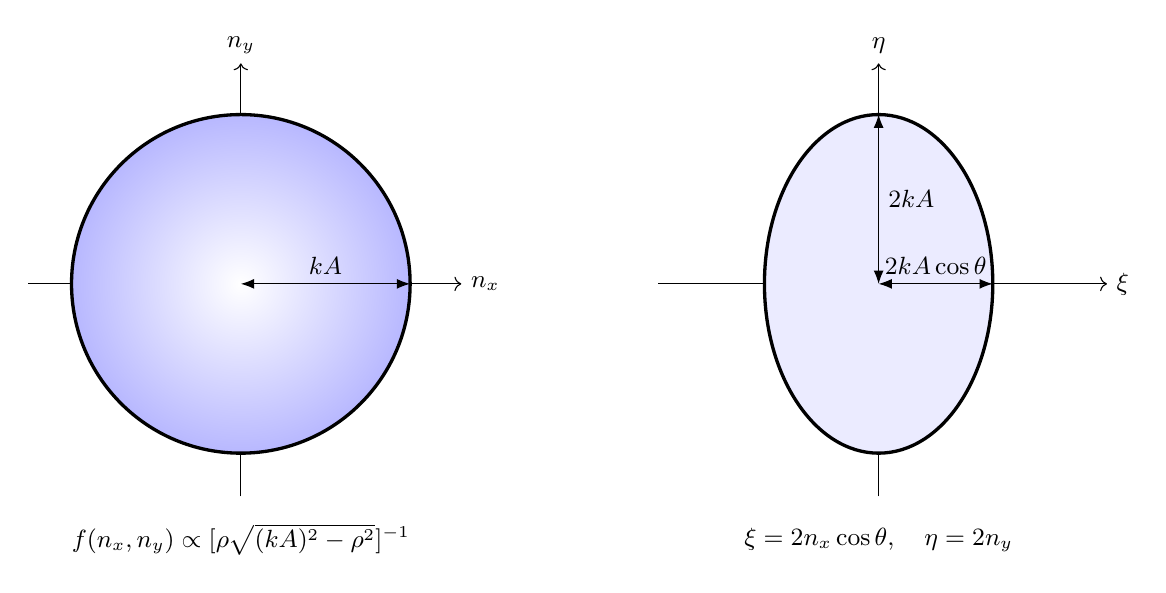
\begin{tikzpicture}[font=\small,x=1cm,y=1cm]
  \begin{scope}[shift={(-4.0,0)}]
    \draw[->] (-2.7,0)--(2.8,0) node[right] {$n_x$}; \draw[->] (0,-2.7)--(0,2.8) node[above] {$n_y$};
    \shade[inner color=white,outer color=blue!28] (0,0) circle (2.15);
    \draw[very thick] (0,0) circle (2.15); \draw[dim] (0,0)--(2.15,0) node[midway,above] {$kA$};
    \node at (0,-3.25) {$f(n_x,n_y)\propto [\rho\sqrt{(kA)^2-\rho^2}]^{-1}$};
  \end{scope}
  \begin{scope}[shift={(4.1,0)}]
    \draw[->] (-2.8,0)--(2.9,0) node[right] {$\xi$}; \draw[->] (0,-2.7)--(0,2.8) node[above] {$\eta$};
    \draw[very thick,fill=blue!8] (0,0) ellipse (1.45 and 2.15);
    \draw[dim] (0,0)--(1.45,0) node[midway,above] {$2kA\cos\theta$};
    \draw[dim] (0,0)--(0,2.15) node[midway,right] {$2kA$};
    \node at (0,-3.25) {$\xi=2n_x\cos\theta,\quad\eta=2n_y$};
  \end{scope}
\end{tikzpicture}

% 15 question-08
\begin{tikzpicture}[x=1.7cm,y=1.3cm,font=\small]

\begin{scope}[x={(.9cm,.12cm)},y={(-.5cm,.36cm)},z={(0cm,.95cm)}]
\foreach\a in{-1,1}\foreach\b in{-1,1}{
\draw[very thick,blue!65](0,0,0)--(\a,\b,0);\fill(\a,\b,0)circle(2pt);
\draw[very thick,red!65](0,0,0)--(\a,0,\b);\fill(\a,0,\b)circle(2pt);
\draw[very thick,green!50!black](0,0,0)--(0,\a,\b);\fill(0,\a,\b)circle(2pt);}
\fill[orange!80](0,0,0)circle(3pt)node[below]{$A$};
\draw[->](0,0,0)--(2.1,0,0)node[right]{$x$};\draw[->](0,0,0)--(0,2.1,0)node[left]{$y$};\draw[->](0,0,0)--(0,0,2)node[above]{$z$};
\end{scope}
\node[align=left,anchor=west]at(3,1){十二个最近邻：\\$(\pm l/2,\pm l/2,0)$\\$(\pm l/2,0,\pm l/2)$\\$(0,\pm l/2,\pm l/2)$};
\node[align=left,anchor=west]at(3,-1.1){$B=(l/2,l/2,0),\ C=(l,0,0)$\\$D=(l,l/2,l/2),\ E=(l,l,0)$\\每条最近邻连线接电阻 $r$};
\end{tikzpicture}

% 16 solution-08
\begin{tikzpicture}[x=1cm,y=1cm,font=\small]

\node[draw,circle](A)at(-4,1){$A$};\node[draw,circle](B)at(-.3,1){$B$};
\draw[resistor](A)--(B)node[midway,above]{$r$};\draw[resistor](A)to[bend right=35]node[midway,below]{$R'=r/5$}(B);
\draw[impulse](-5.4,1)--(A)node[midway,above]{$I$};\node at(-2.2,-1){$R_{AB}=r\parallel(r/5)=r/6$};
\node[draw,circle](B2)at(2.1,1){$B$};
\foreach\y/\lab in{2.5/{2\times C},1/{4\times D},-.5/{1\times E}}{\draw[resistor](B2)--(5,\y)node[right]{$\lab$};}
\node[align=center]at(3.5,-1.7){其余四个邻点与 $B$ 等势\\$I/12=2I_{BC}+4I_{BD}+I_{BE}$\\$2R_{AC}+4R_{AD}+R_{AE}=4r/3$};
\end{tikzpicture}

\end{document}
